\section{Results}
All the implemented transforms where tested for correctness by comparing the output
of my implementation to other reference-implementations, like matlab's or scipy's.
The implementation was also tested for speed depending on the length of the input.
For a given input length the FFT algorithm was performed multiple times with random numbers
and the
runtime was measured and averaged. The number of times the algorithm was evaluated
was chosen, such that the uncertainty of the average was below \SI{10}{\nano\second}.
While the actual numbers will be more or less uninteresting, it is possible to see
the $\symcal{O}(N\log N)$ scaling for powers of 2, as shown in \autoref{fig:timesp2}.
Especially for higher-length input the scaling is fulfilled, but for short length
input there is too much overhead, and thus the numbers are not following $N\log N$ perfectly there.

\begin{figure}[t]
    \centering
    \includegraphics[width=\linewidth]{build/plots/times_p2.pdf}
    \caption{Runtime of my FFT implementation in double-logarithmic-scaling depending on the length of the input sequence.
        Each random-number input is transformed multiple time and the results were averaged.
        The function $t(N)=c\times N\log N$ is fitted to the measurements, as we expect this scaling for
        input lengths in the form of $2^p$. }
    \label{fig:timesp2}
\end{figure}

For arbitrary sized input, the actual runtime of this algorithm depends heavily on
the number of two's in the prime-factor decomposition of the input-length.
In easier words: the FFT of 48 numbers should be roughly twice as fast as 56, even though
56 is the higher number.
The reason is 48 is divisible by 2 4 times ($48=2^4\cdot 3$), where 56 is only divisble by
2 3 times ($56=2^3\cdot 7$).
This is also clearly seen in the data, as \autoref{fig:times} shows.
\begin{figure}[t]
    \centering
    \includegraphics[width=.5\textwidth]{build/plots/times_lin_c.pdf}
    \caption{Averaged runtime of the implemented FFT algorithm on random numbers depending on the input length.
        A clear separation of the runtime scaling is seen. The data-points are colored
        depending on the number of times the input length is divisible by 2.}
    \label{fig:times}
\end{figure}


\subsection{Depicting the Fourier Space}
A digital image is nothing more than $N=h\cdot w\cdot C$ numbers $x_{k,l,c}$
\footnote{$k=0,\dots, h-1\quad l=0,\dots,w-1\quad c=0,\dots,C-1$}
between $0$ and $1$.
Where $w$ is the width, $h$ is the height and $C$ is the number of channels of the image.
There are a lot of different types of images out there, with different channel numbers and interpretation
of them (different color encodings, transparent images, etc.), but we will focus on the
case of grayscale $C=1$ or colored RGB $C=3$ pictures.
The interpretation of the number in grayscale images is the illumination of the pixel ranging from $0=$~off~$=$~black
to $1=$~on~$=$~white.
In colored RGB images, we have three channels: Red (R), Green (G), Blue (B). Where we can light up each color separately.
Because of how the eye works, we are able to trick the brain into perceiving most of the colors by just
mixing these three.
The numbers are usually not stored as floating point numbers, but as unsigned integers, most commonly 8-bit unsigned integers.
This means that 1 is stored as 255 and 0 as 0 and all the numbers are mapped in an equally spaced fashion.
If we have multiple channels, we will Fourier transform each channel separately and
equation \eqref{eqn:dft2d} gets the form
\begin{equation*}
    X_{k,l,c} = \frac{1}{\sqrt{hw}}\sum_{n=0}^{h-1}\sum_{m=0}^{w-1}x_{n,m,c} \ e^{-i{2\pi}\ \left(\!\frac{kn}{h}+\frac{lm}{w}\right)}.
\end{equation*}
In the Fourier space each pixel is a complex number.
We usually visualize the magnitude and the phase (the argument) of each number.
Because the magnitude of the Fourier transformed numbers is not guaranteed
to be between 0 and 255, we scale the Fourier transformed numbers in such a way,
that the highest is 255 and the lowest is 0
\begin{equation*}
    \abs {X'_{k,l,c}} = 255\frac{\abs {X_{k,l,c}}-\min_{n,m} \abs {X_{n,m,c}}}{\max_{n,m} \abs {X_w{n,m,c}}-\min_{n,m} \abs {X_{n,m,c}}}.
\end{equation*}
We also scale the phases to the range of $(0, 255)$
\begin{equation*}
    \arg {X'_{k,l,c}} = 255\frac{\arg X_{k,l,c}}{2\pi}.
\end{equation*}
This mode of visualization can be seen in \autoref{subfig:ftm_n} and \autoref{subfig:ftp_n}.
\begin{figure}[htbp]
    \centering
    \begin{subfigure}[h]{.9\linewidth}
        \centering
        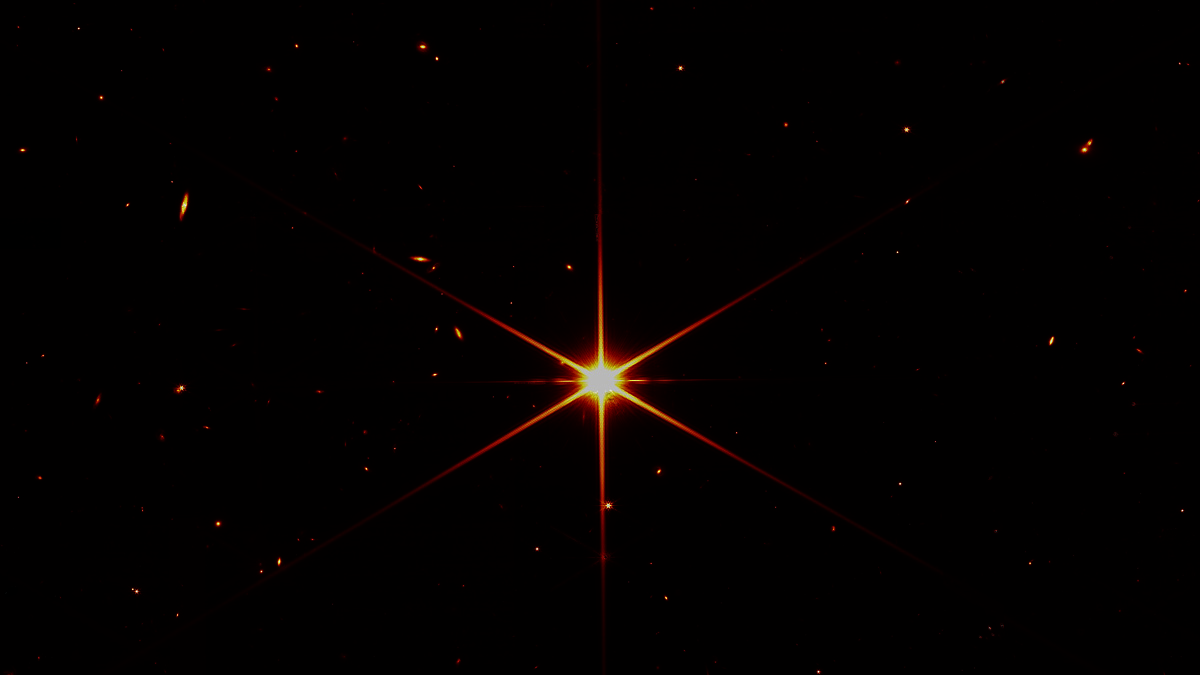
\includegraphics[width=\linewidth]{images/webb.png}
        \caption{Original}
    \end{subfigure}
    \begin{subfigure}[h]{.9\linewidth}
        \centering
        \includegraphics[width=\linewidth]{build/output/webb_mag_n.png}
        \caption{Fourier Transform Magnitude}
        \label{subfig:ftm_n}
    \end{subfigure}
    \begin{subfigure}[h]{.9\linewidth}
        \centering
        \includegraphics[width=\linewidth]{build/output/webb_phase_n.png}
        \caption{Fourier Transform Phase}
        \label{subfig:ftp_n}
    \end{subfigure}
    \begin{subfigure}[h]{.9\linewidth}
        \centering
        \includegraphics[width=\linewidth]{build/output/webb_mag_log.png}
        \caption{Fourier Transform magnitude in logarithmic space}
        \label{subfig:ftm_log}
    \end{subfigure}
    \begin{subfigure}[h]{.9\linewidth}
        \centering
        \includegraphics[width=\linewidth]{build/output/webb_mag.png}
        \caption{FT Magnitude in logarithmic space and rearranged}
        \label{subfig:ftm}
    \end{subfigure}
    \caption{An example of the Fourier transform. The image is the first calibration picture of the new James-Webb space telescope\cite{webbimg}. }
    \label{fig:fourier_example_n}
\end{figure}

As you can see in the example image, the Fourier magnitude is mostly black, and the phases appear to be noise to the eye.
To better distinguish small features, we will now switch to logarithmic color-space for the magnitude
\begin{equation*}
    \abs {X''_{k,l,c}} = 255\frac{\log \abs {X_{k,l,c}}-\min_{n,m} \log\abs {X_{n,m,c}} } {\max_{n,m} \log\abs {X_{n,m,c}}-\min_{n,m} \log\abs {X_{n,m,c}}}.
\end{equation*}
This is depicted in \autoref{subfig:ftm_log}.
Finally, to better resemble the symmetries in the Fourier space and
to have low frequencies in the middle of the picture, and high frequencies outside,
the indices are shifted
\begin{equation}
    k' = \lfloor k+h/2\rfloor \mod h \qquad l'=\lfloor l+w/2\rfloor\mod w.
    \label{eqn:shift}
\end{equation}
This will be our method of visualization from now on and can be seen in \autoref{subfig:ftm}.

\subsection{Editing in Fourier Space}
If we now modify the numbers in the Fourier space and transform the modified numbers back,
we can achieve complex-looking outcome.
For example, if we take the high frequencies in the image away, we are only left with the
"long-range" information, but the "short-range" information is lost.
This means the image will appear to be blurred.
Taking away the high frequencies can be done in multiple ways.
We can just remove the highest frequencies combining the axes by calculating
$(k'-h/2)^2+(l'-w/2)^2 < r^2$ for some $r$ and setting the pixel in Fourier space to 0, if
this evaluates to false. We can also do this for each axis independently
($(k'-h/2)^2<r_y^2$, $(l'-w/2)^2<r_x^2$).
With these hard cut-offs it is easy to see periodic artifacts in the image.
If we do not want that, we can apply a smooth filter.
A selection of different blurring techniques can be seen
in \autoref{fig:blur_2} to \autoref{fig:blur_smooth}.

\begin{figure}[htbp]
    \centering
    \begin{subfigure}[h]{.49\linewidth}
        \centering
        \includegraphics[width=.9\linewidth]{build/output/dune_mag.png}
        \caption{Fourier space}
    \end{subfigure}
    \begin{subfigure}[h]{.49\linewidth}
        \centering
        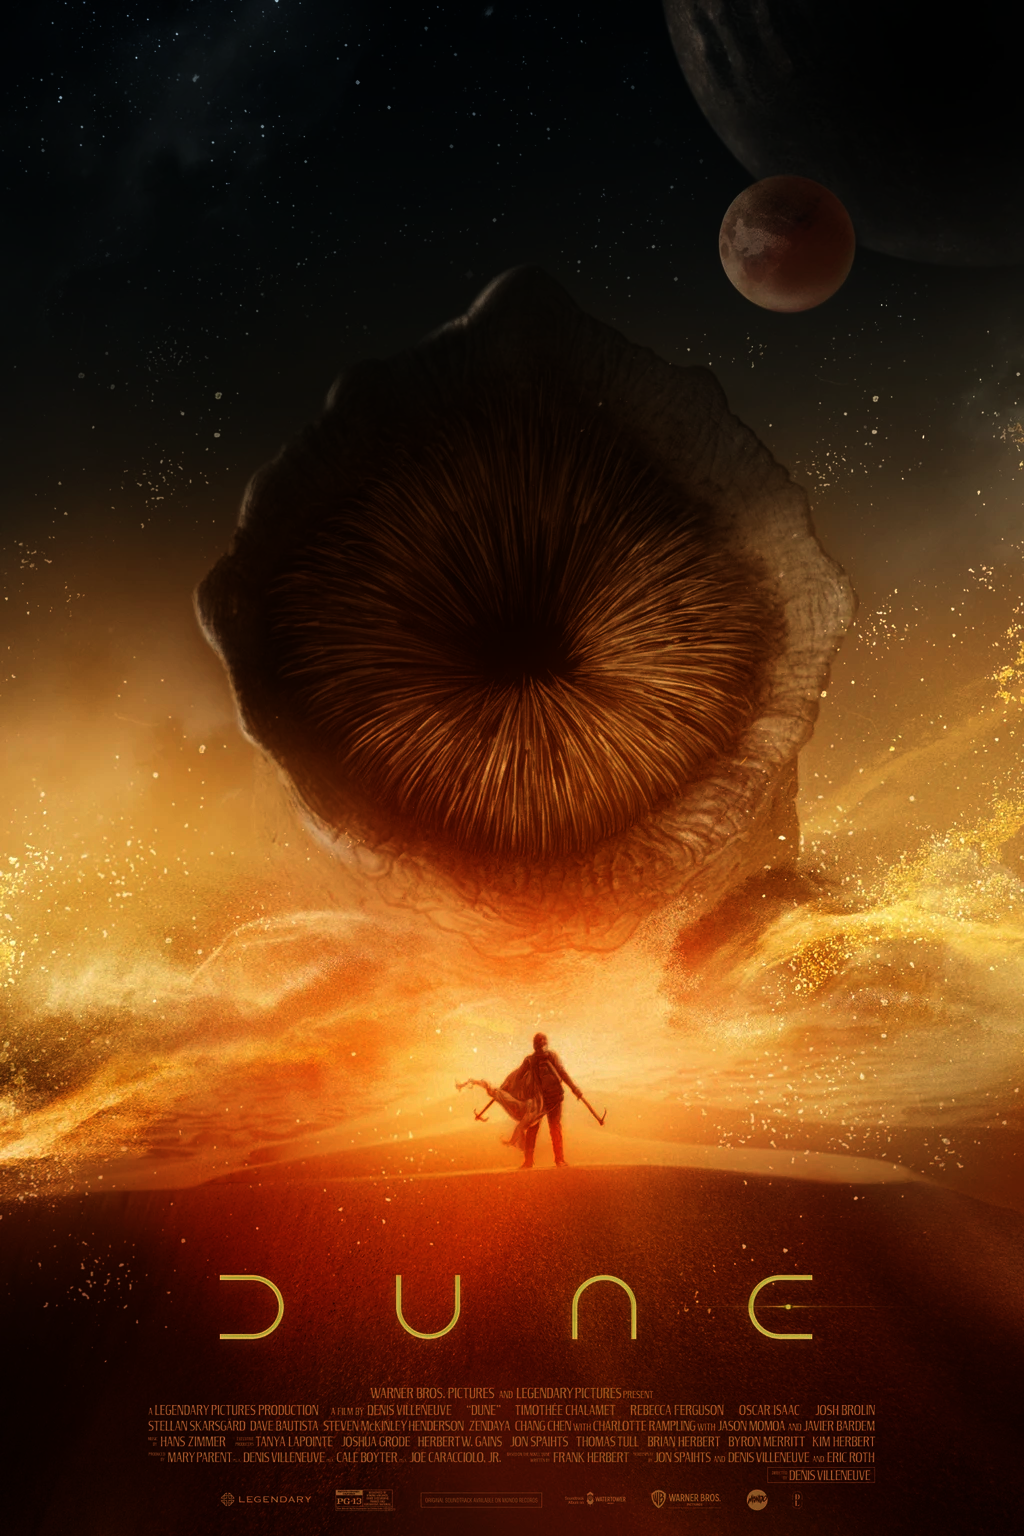
\includegraphics[width=.9\linewidth]{images/dune.png}
        \caption{Original}
    \end{subfigure}\
    \caption{A movie poster of Dune (2021) which serves as an example image being blurred in this section \cite{dune}.}
    \label{fig:dune_orig}
\end{figure}

\begin{figure}[htbp]
    \centering
    \begin{subfigure}[h]{.49\linewidth}
        \centering
        \includegraphics[width=.9\linewidth]{build/output/dune_blur2_mask.png}
        \caption{Edit in Fourier space }
    \end{subfigure}
    \begin{subfigure}[h]{.49\linewidth}
        \centering
        \includegraphics[width=.9\linewidth]{build/output/dune_blur2.png}
        \caption{Transformed back to real space}
    \end{subfigure}\
    \caption{The poster above blurred by only keeping the innermost frequencies with a radius of $20\%$ of the width.}
    \label{fig:blur_2}
\end{figure}
\begin{figure}[htbp]
    \centering
    \begin{subfigure}[h]{.49\linewidth}
        \centering
        \includegraphics[width=.9\linewidth]{build/output/dune_blur1_mask.png}
        \caption{Edit in Fourier space }
    \end{subfigure}
    \begin{subfigure}[h]{.49\linewidth}
        \centering
        \includegraphics[width=.9\linewidth]{build/output/dune_blur1.png}
        \caption{Transformed back to real space}
    \end{subfigure}\
    \caption{The poster blurred by only keeping the innermost frequencies with a radius of $10\%$ of the width. This is a circular filter.}
    \label{fig:blur_1}
\end{figure}
\begin{figure}[htbp]
    \centering
    \begin{subfigure}[h]{.49\linewidth}
        \centering
        \includegraphics[width=.9\linewidth]{build/output/dune_rect_mask.png}
        \caption{Edit in Fourier space }
    \end{subfigure}
    \begin{subfigure}[h]{.49\linewidth}
        \centering
        \includegraphics[width=.9\linewidth]{build/output/dune_blur_rect.png}
        \caption{Transformed back to real space}
    \end{subfigure}\
    \caption{The poster blurred by only keeping the $10\%$ innermost frequencies along each axis independently. This is a rectangular filter.}
    \label{fig:blur_rect}
\end{figure}
\begin{figure}[htbp]
    \centering
    \begin{subfigure}[h]{.49\linewidth}
        \centering
        \includegraphics[width=.9\linewidth]{build/output/dune_blur_smooth_mask.png}
        \caption{Edit in Fourier space }
    \end{subfigure}
    \begin{subfigure}[h]{.49\linewidth}
        \centering
        \includegraphics[width=.9\linewidth]{build/output/dune_blur_smooth.png}
        \caption{Transformed back to real space}
    \end{subfigure}\
    \caption{The poster blurred by only multipliying each pixel in the Fourier space with $\exp(-0.001 ((k'-h/2)^2+(l'-w/2)^2))$, where $k', l'$ are the shifted indices from above. This is a Gaussian filter.}
    \label{fig:blur_smooth}
\end{figure}

\FloatBarrier

If we do the opposite and take away some low frequencies, we are "sharpening" the image.
We must not understand "sharpening" in the literal meaning, like focusing the lens of a camera,
since we can not generate new information in the image. We can only enhance the short range information.
There are a couple of examples below in \autoref{fig:blackhole} to \autoref{fig:blackhole_sharp_g_g}.
You will notice the colors in the images are distorted, since we completely treat the
color channels separately. In \autoref{fig:blackhole_sharp_g_g} you can see a grayscale version
of the edit, where the colors might be less distracting.

If we take it to the extreme and remove most low frequencies, we can seethe edges in the image, this
is demonstrated in \autoref{fig:edges}.
\begin{figure}
    \centering
    \begin{subfigure}[h]{.49\linewidth}
        \centering
        \includegraphics[width=.9\linewidth]{build/output/blackhole_sharp_smooth_mask.png}
        \caption{Fourier space}
    \end{subfigure}
    \begin{subfigure}[h]{.49\linewidth}
        \centering
        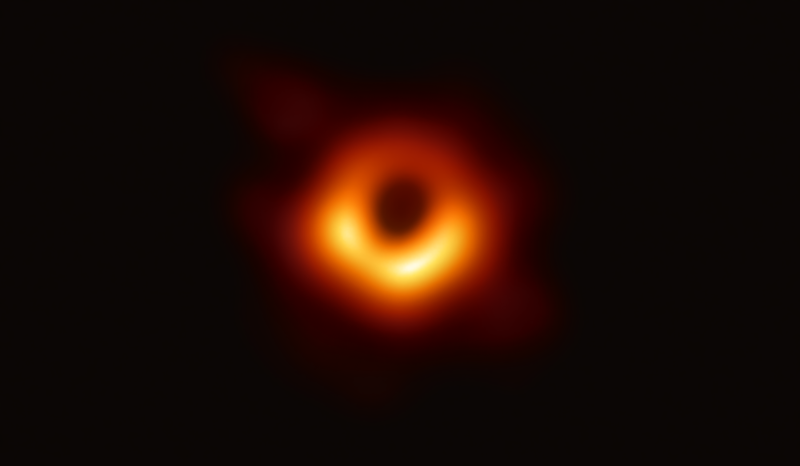
\includegraphics[width=.9\linewidth]{images/blackhole.png}
        \caption{Original}
    \end{subfigure}\
    \caption{The first image of a black hole, taken in 2021.
        This appears not to be sharp and is taken as an example to experiment with sharpening in Fourier space in this section. }
    \label{fig:blackhole}
\end{figure}
\begin{figure}
    \centering
    \begin{subfigure}[h]{.49\linewidth}
        \centering
        \includegraphics[width=.9\linewidth]{build/output/blackhole_sharp1_mask.png}
        \caption{Edit in Fourier space}
    \end{subfigure}
    \begin{subfigure}[h]{.49\linewidth}
        \centering
        \includegraphics[width=.9\linewidth]{build/output/blackhole_sharp1.png}
        \caption{Transformed back to real space}
    \end{subfigure}\
    \caption{The black hole image sharpened by applying a circular filter with a radius of 1\% of the height.}
    \label{fig:blackhole_sharp}
\end{figure}
\begin{figure}
    \centering
    \begin{subfigure}[h]{.49\linewidth}
        \centering
        \includegraphics[width=.9\linewidth]{build/output/blackhole_sharp3_mask.png}
        \caption{Edit in Fourier space}
    \end{subfigure}
    \begin{subfigure}[h]{.49\linewidth}
        \centering
        \includegraphics[width=.9\linewidth]{build/output/blackhole_sharp3.png}
        \caption{Transformed back to real space}
    \end{subfigure}\
    \caption{The black hole image sharpened by applying a circular filter with a radius of 3\% of the height.}
    \label{fig:blackhole_sharp3}
\end{figure}
\begin{figure}
    \centering
    \begin{subfigure}[h]{.49\linewidth}
        \centering
        \includegraphics[width=.9\linewidth]{build/output/blackhole_sharp_smooth_mask.png}
        \caption{Edit in Fourier space}
    \end{subfigure}
    \begin{subfigure}[h]{.49\linewidth}
        \centering
        \includegraphics[width=.9\linewidth]{build/output/blackhole_sharp_smooth.png}
        \caption{Transformed back to real space}
    \end{subfigure}\
    \caption{The black hole image sharpened by applying a Gaussian filter of $1-\exp(-0.01 ((k'-h/2)^2+(l'-w/2)^2))$.}
    \label{fig:blackhole_sharp_g}
\end{figure}
\begin{figure}
    \centering
    \begin{subfigure}[h]{.49\linewidth}
        \centering
        \includegraphics[width=.9\linewidth]{build/output/blackhole_sharp_smooth_mask_g.png}
        \caption{Edit in Fourier space}
    \end{subfigure}
    \begin{subfigure}[h]{.49\linewidth}
        \centering
        \includegraphics[width=.9\linewidth]{build/output/blackhole_sharp_smooth_g.png}
        \caption{Original}
    \end{subfigure}\
    \caption{The black hole image sharpened by applying a Gaussian filter of $1-\exp(-0.01 ((k'-h/2)^2+(l'-w/2)^2))$ in black and white.}
    \label{fig:blackhole_sharp_g_g}
\end{figure}
\begin{figure}
    \centering
    \begin{subfigure}[h]{.32\linewidth}
        \centering
        
\includegraphics[width=.9\linewidth]{images/A.png}
        \caption{Original }
    \end{subfigure}
    \begin{subfigure}[h]{.32\linewidth}
        \centering
        \includegraphics[width=.9\linewidth]{build/output/A_sharp_smooth_mask.png}
        \caption{Edit}
    \end{subfigure}
    \begin{subfigure}[h]{.32\linewidth}
        \centering
        \includegraphics[width=.9\linewidth]{build/output/A_sharp_smooth.png}
        \caption{Back to real space}
    \end{subfigure}
    \caption{An image sharpened with a Gaussian filter of $1-\exp(-0.001 ((k'-h/2)^2+(l'-w/2)^2))$ to demonstrate edge-detecting capabilities of Fourier edits.}
    \label{fig:edges}
\end{figure}
\FloatBarrier

\subsection{Diffraction}
As already mentioned, we can
"simulate" Fraunhofer diffraction by displaying the magnitude of the Fourier transformed image.
In the images in this section, you will be able to realize a couple of known features
of diffraction images.
Lines in the diffraction images will be perpendicular to lines in the aperture (the original image).
For two double slits of width $b$ and distance $a$ the analytical expression for Fraunhofer diffraction
is
\begin{equation*}
    I(\theta) = I_0 \left(\frac{\sin(c b \sin\theta)}{c b \sin\theta} \cos(c a \sin\theta)\right)^2.
\end{equation*}
Which is calculated by solving equation \eqref{eqn:fraunhofer}.
With some constant $c$. From this we can read that the smaller the slits are, the wider the
encapsulating intensity is (since $b < a$) and the closer the slits are, the smaller the distance between
the peaks is. This can be seen in \autoref{fig:double_slit}.

This calculation is rather simple, but also more complex apertures can be investigated, like a circular
aperture, seen in \autoref{fig:circular}. The analytical solution to this is a Bessel function of the radius.

\begin{figure}[htbp]
    \centering
    \begin{subfigure}[h]{\linewidth}
        \centering
        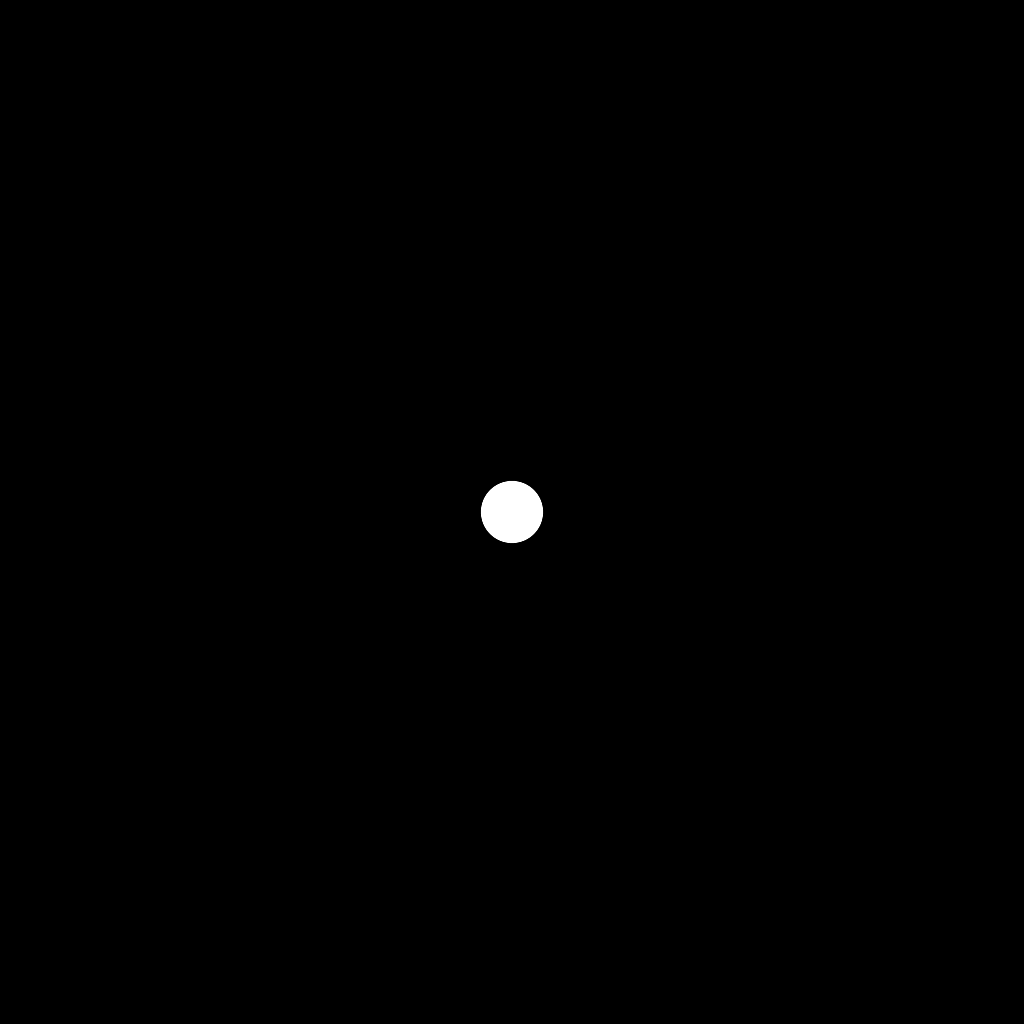
\includegraphics[width=.49\linewidth]{images/hole.png}
        \includegraphics[width=.49\linewidth]{build/output/hole_mag.png}
        \caption{Circular aperture.}
    \end{subfigure}
    \begin{subfigure}[h]{\linewidth}
        \centering
        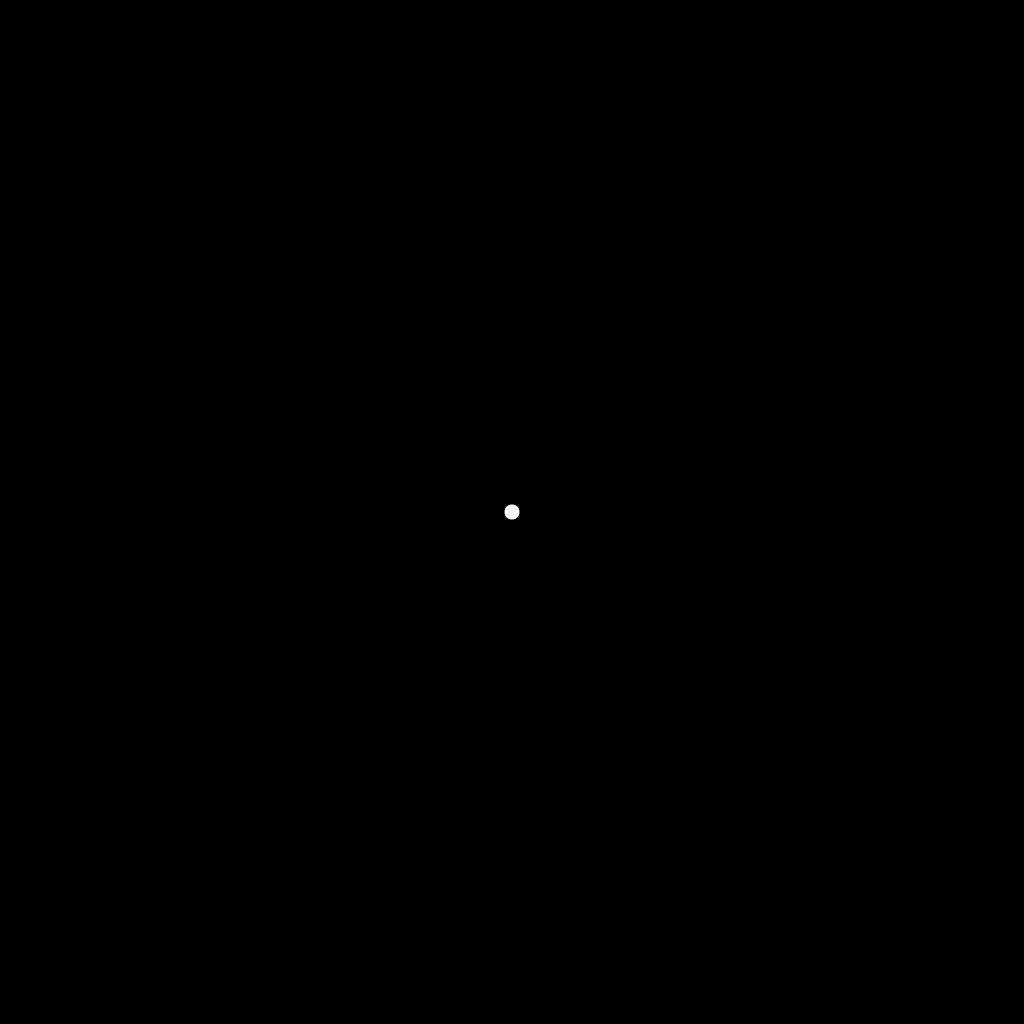
\includegraphics[width=.49\linewidth]{images/hole_tiny.png}
        \includegraphics[width=.49\linewidth]{build/output/hole_tiny_mag.png}
        \caption{Circular aperture with smaller radius.}
    \end{subfigure}
    \caption{Fraunhofer diffraction image (right) for two different circular apertures (left).}
    \label{fig:circular}
\end{figure}


\begin{figure}[htbp]
    \centering
    \begin{subfigure}[h]{\linewidth}
        \centering
        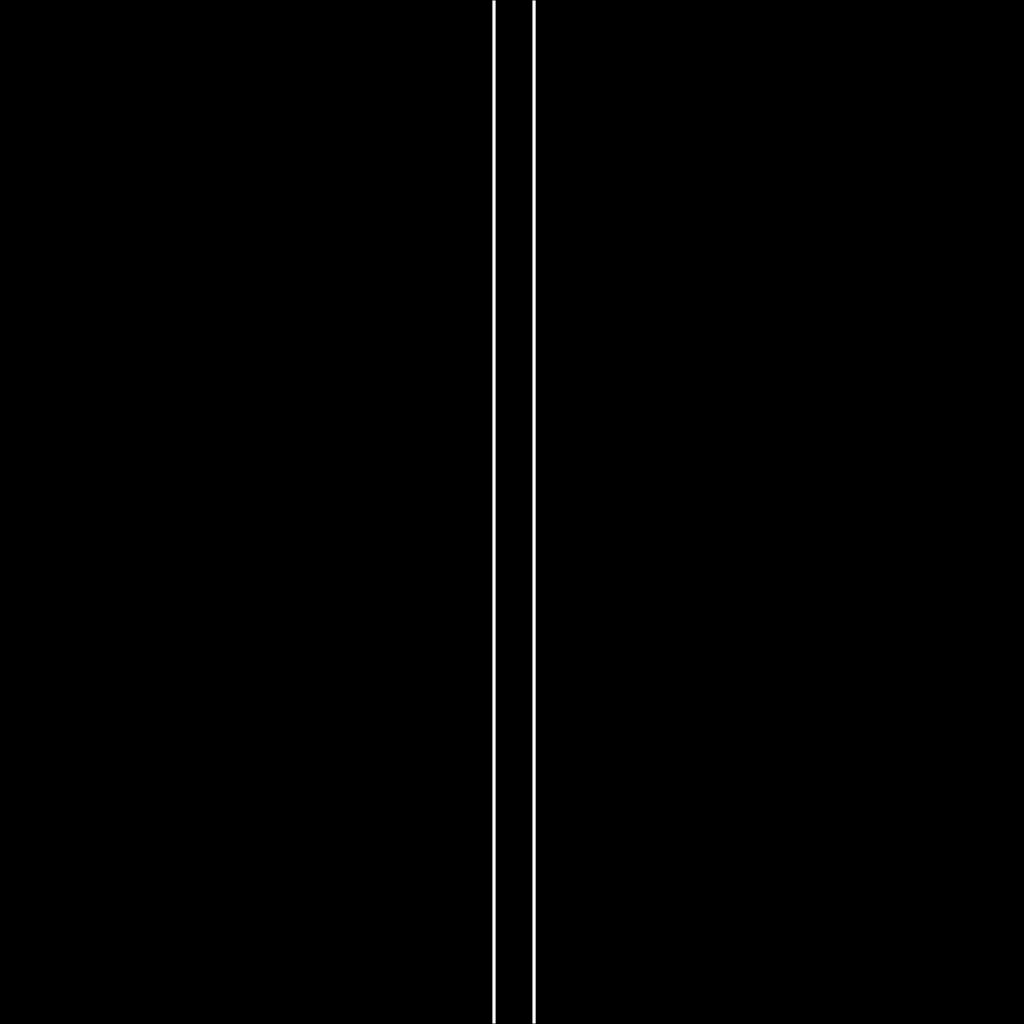
\includegraphics[width=.49\linewidth]{images/double_slit_small_norm.png}
        \includegraphics[width=.49\linewidth]{build/output/double_slit_small_norm_mag.png}
        \caption{Double slit.}
    \end{subfigure}
    \begin{subfigure}[h]{\linewidth}
        \centering
        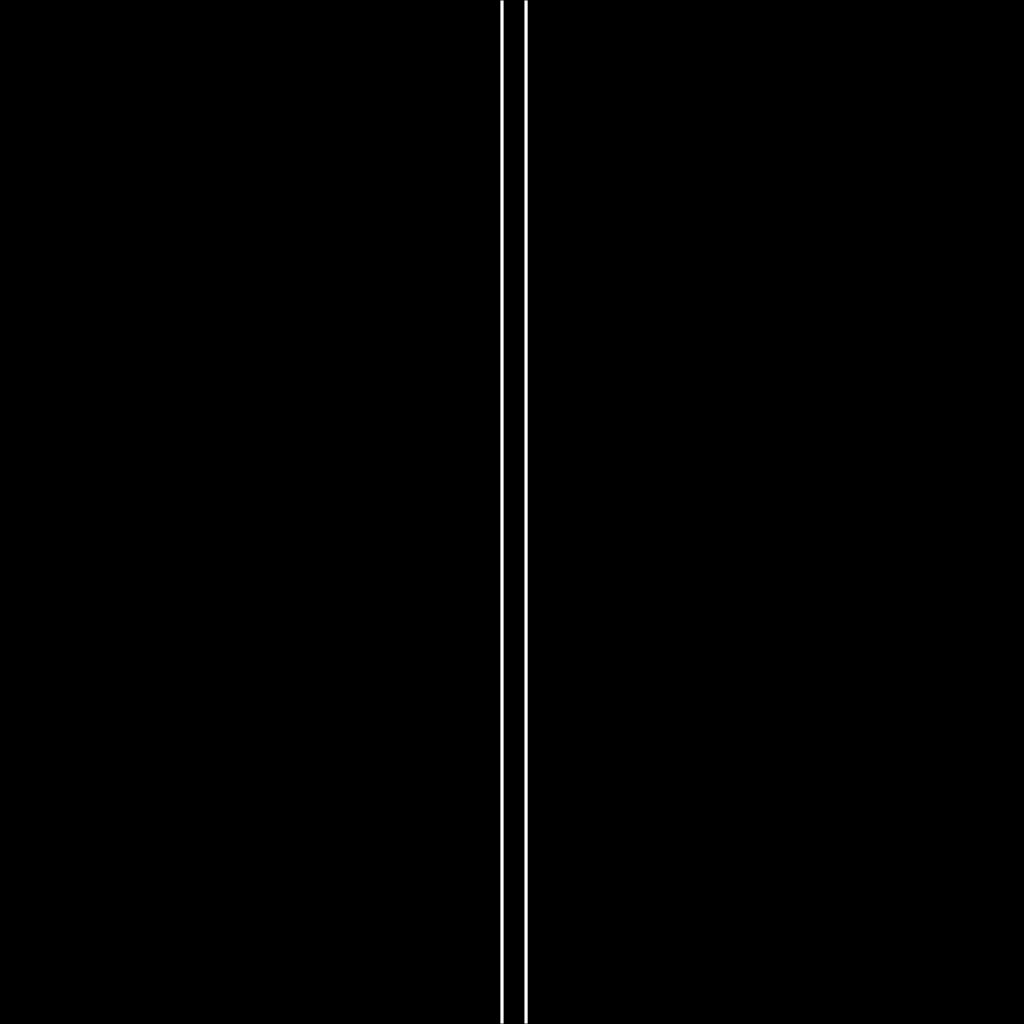
\includegraphics[width=.49\linewidth]{images/double_slit_small_close.png}
        \includegraphics[width=.49\linewidth]{build/output/double_slit_small_close_mag.png}
        \caption{Double slit where the slits are closer.}
    \end{subfigure}
    % \begin{subfigure}[h]{\linewidth}
    %     \centering
    %     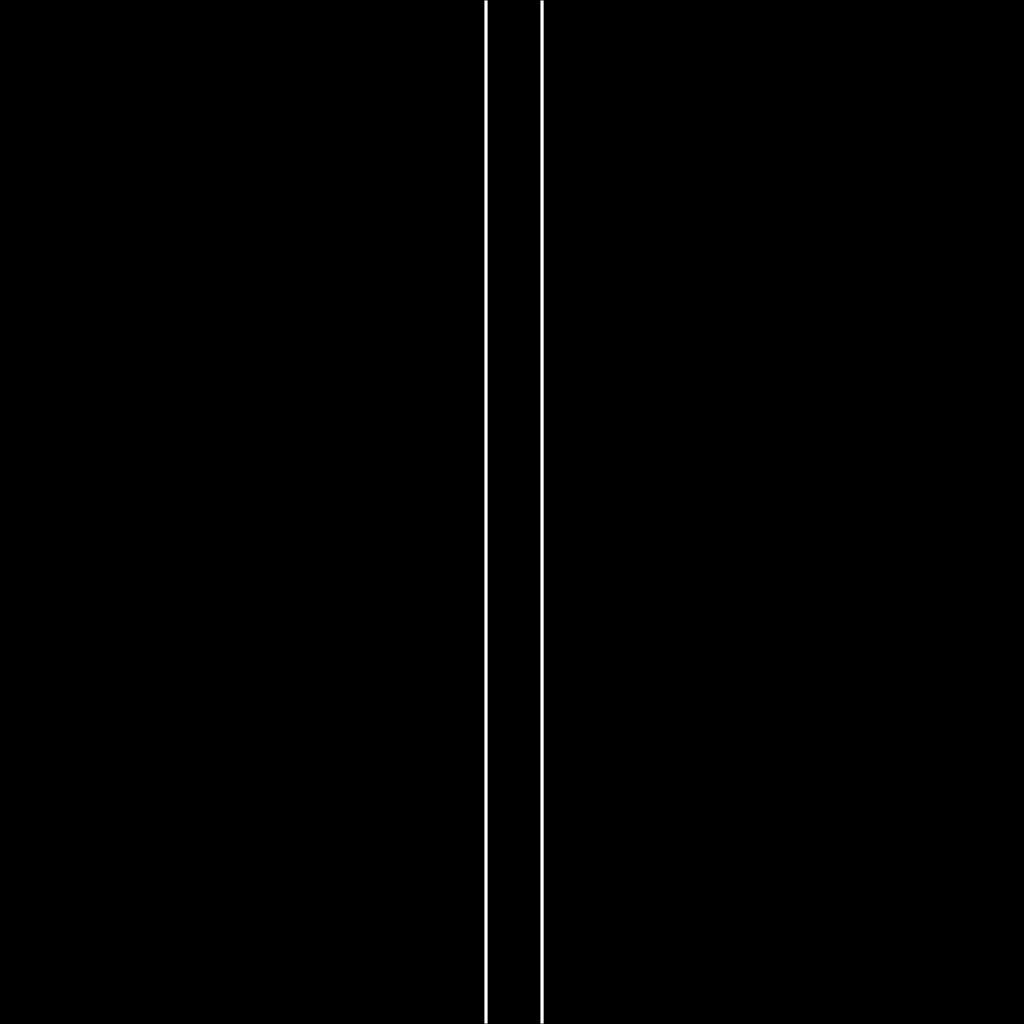
\includegraphics[width=.49\linewidth]{images/double_slit_small_wide.png}
    %     \includegraphics[width=.49\linewidth]{build/output/double_slit_small_wide_mag.png}
    %     \caption{Simulated diffraction image (right) of aperture image (left).}
    % \end{subfigure}
    \begin{subfigure}[h]{\linewidth}
        \centering
        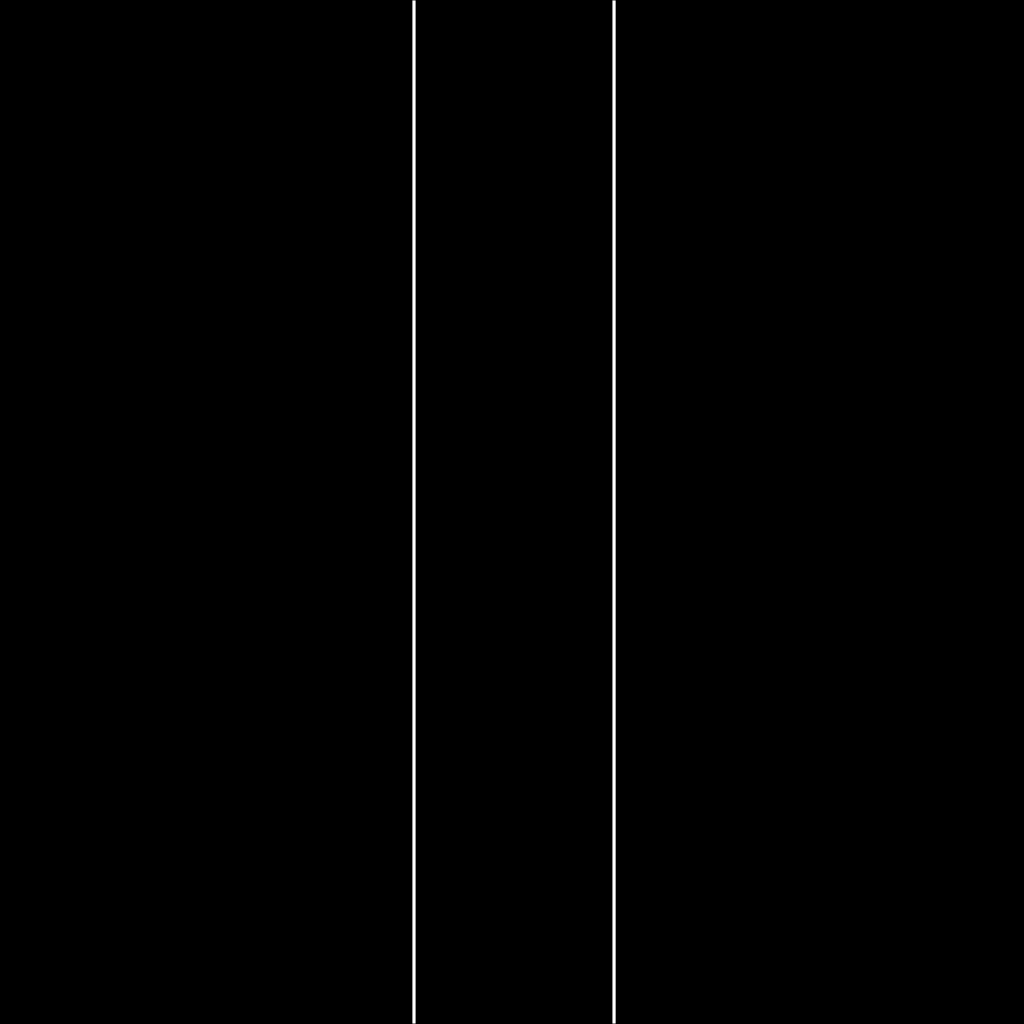
\includegraphics[width=.49\linewidth]{images/double_slit_small_widest.png}
        \includegraphics[width=.49\linewidth]{build/output/double_slit_small_widest_mag.png}
        \caption{Double slit where the slits are further apart.}
    \end{subfigure}
    \begin{subfigure}[h]{\linewidth}
        \centering
        
\includegraphics[width=.49\linewidth]{images/double_slit_norm_widest.png}
        \includegraphics[width=.49\linewidth]{build/output/double_slit_norm_widest_mag.png}
        \caption{Double slit with wider slits, but same distance as last image.}
    \end{subfigure}
    \caption{Different images of double slits with different features. The aperture image is on the left and the diffraction image is on the right.}
    \label{fig:double_slit}
\end{figure}

\subsection{Compression}
In this section we will very quickly review a naive compression algorithm, based on the discrete cosine transform.
Here the images will not be displayed in the transformed space, since they were very uninformative in my testing.
They appeared to look like mostly a single color with very subtle variation.
The idea of our naive compression is to sort the cosine-space coefficient by magnitude and just
set the lowest of them to zero. Then we only need to save the nonzero coefficients.
The results of removing the lowest coefficients in this way can be seen in \autoref{fig:compr}.

It is fairly obvious, that this compression is not looking very good, except at low compression rates.
But would it save space on disk? To answer this question I implemented a very simple binary format,
saving the cosine coefficients and their indices in a binary, compressed format. Sadly, except
at absurdly high compressions, this did not save disk space.
On the contrary: The file size actually increased, since now that we are not saving every
pixel, we also have to save the indices, which takes additional space.
The actual \texttt{.jpg} format is a little bit more complicated.
It performs the DCT on each $8\times 8$ tile in the image and instead of
setting small amplitudes to 0, it tries to find a smaller, finite set of amplitudes,
so that setting the real amplitudes to the one closest to it in the smaller set of amplitudes, does
not change too much.
\begin{figure}[htbp]
    \centering
    \begin{subfigure}[h]{.49\linewidth}
        \centering
        \includegraphics[width=\linewidth]{build/plots/A9.png}
        \caption{10\% compression}
    \end{subfigure}
    \begin{subfigure}[h]{.49\linewidth}
        \centering
        \includegraphics[width=\linewidth]{build/plots/A5.png}
        \caption{50\% compression}
    \end{subfigure}
    \begin{subfigure}[h]{.49\linewidth}
        \centering
        \includegraphics[width=\linewidth]{build/plots/A2.png}
        \caption{80\% compression}
    \end{subfigure}
    \begin{subfigure}[h]{.49\linewidth}
        \centering
        \includegraphics[width=\linewidth]{build/plots/A1.png}
        \caption{90\% compression}
    \end{subfigure}
    \caption{The same image with different "compression levels". 10\% compression means that the lowest 10\% of the
        cosine coefficients have been set to 0.}
    \label{fig:compr}
\end{figure}